% !TEX encoding = UTF-8 Unicode
\chapter{Introduction}
\label{chp: chap1}

\section{Background}
Selon le rapport de l'enquête sur la criminalité et la sécurité de CSI Computer en 2010 et 2011, 92 pourcent des entreprises ont souffert d'une attaque d'application réussie entre Juillet 2009 et Juin 2010. Pire encore selon William Noonan [Richardson, 2010/2011], la fréquence et la complexité des crimes cybernétiques ont augmenté de manière significative. En plus, 69 pourcent des répondants américains ont souligné que l'impact des cyber-menaces à leur entreprise a attiré leur attention (contre 49 pour cent l'année précédente). La situation ci-dessus illustre l'importance de la sécurité dans les affaires en particulier dans les serveurs Web. En outre, d'autres produits logiciels sont construits sur le web infrastructure que l'application native. Surtout, une nouvelle page pour l'application Web,  le développement a été tourné quand Roy Thomas Fielding a présenté la nouvelle architecture  Web REST nommée ( Representational State Transfer) dans le chapitre 5 de son doctorat  intitulée "Architectural Styles and the Design of Network-based Software Architectures". Ceci est la raison de la croissance importante des API [Hughes Systique Coporation, 2006]. La nouvelle architecture peut favoriser un meilleur environnement pour le développement d’un site Web, cependant, elle apporte aussi de nouveaux défis en matière de sécurité qui doit être adapté dans la nouvelle infrastructure. Ainsi, ce mémoire de master explore comment marche les méthodes de sécurité des services web rest avec les sites web.
Ce mémoire a pour but d'examiner les deux domaines suivantes :
\begin{itemize}
\item Comment les serveurs de Twitter et Stripe authentifient les requêtes provenant de divers applications clientes.
\item Comment les sites web exploitent les API afin de améliorer l'environnement web pour le e-commerce.
\end{itemize}
Sur la base des deux questions mentionnées ci-dessus, cette recherche est divisé en deux grandes parties. La première partie (chapitres 1- 5) centré sur la première champ. La deuxième partie (chapitre 6) fournit la solution et répond à la deuxième champ en utilisant un site Web et un framework Python conçus par l'auteur, qui peut aider les utilisateurs à faire des appels API d'une manière simple et maintenir l'intégrité des services.
Avant de passer au chapitre suivant, il est nécessaire de définir les termes de base et
concepts utilisés dans la thèse.

\section{Définitions des termes et concepts}
\begin{itemize}
\item[•]  Site web intégré : le concept de base des sites web intégrés est de fournir plusieurs outils et services qui utilisent différentes technologies et qui sont fournis par plusieurs services web. En utilisant des sites web intégrés du coté client, les utilisateurs sont capables d'interagir, de coopérer et de consumer plusieurs services web héberges dans différents serveurs.

\item  API : (Application program interface)  est un ensemble d'outils,  de fonctions et de protocoles dont les utilisateurs peuvent se référer et les intégrer dans le développement de leur applications.

\item  Sécurité web: Cela implique comment définir des principes pour protéger les services web et les clients web. Mais aussi comment déterminer les vulnérabilités du  système dans tous les étapes du processus tel que le développement, l'analyse des besoins, la conception et la maintenance des applications. Selon la CIA triad, il y a trois principales composantes qui sont cruciaux pour la sécurité web :
 \begin{itemize}
 \item Intégrité : C'est le principe qui stipule que les données doivent être correct. Certains accès non authentifié pourrait causer des modifications inattendues des données, par exemple, les données d'utilisateur été changé au cours de la transaction par un tiers [Cryptome, 2013]. 
 \item Confidentialité : Les données d'un utilisateur ont été espionnées à la fois du côté serveur et côté client. Cela pourrait conduire à la perte de la vie privée de l'utilisateur. Ainsi, chaque accès devrait être attentivement  autorisé [Hall, 2005]. Dans ce cas, les données provenant de faux utilisateurs  peuvent passer par tous les processus d'authentification et deviennent valides. Par conséquent, les faux utilisateurs peuvent envoyer de demandes erronées au nom des victimes. Ceci est dangereux tant pour les services et la utilisateurs; Par conséquent, cette thèse analyse également certains processus d'authentification qui sont utilisé par les fournisseurs de l'API.
 \item La disponibilité : Ceci fait référence à l'accessibilité des données. Cela signifie que l'information doit être disponible quand il est nécessaire. Par conséquent, les mécanismes d'authentification, les voies d'accès et le matériel doivent fonctionner correctement. Cela fonctionne contre les actions malveillantes telles que le déni de service. Les serveurs web peuvent être attaqués de différentes manières comme les attaques DoS, le bourrage de mémoire etc … Ce genre de menace peut causer des lenteurs inattendu durant les transferts de donnée entre le client et serveur, ou pire cela pourrait endommagé le serveur.
 \end{itemize}
\end{itemize}
 Présentement il existe plusieurs méthodes de sécurité. Cependant, toutes ces méthodes peuvent être classées dans une ou plusieurs des catégories suivantes.
 \begin{itemize}
 \item Domain Based Security Model (DBSy) : Il a été crée vers la fin des années 90 par Defense Evalution and Research Agency (DERA). C'est un ensemble de notations et de techniques développés spécialement pour le gouvernement britannique par par QinetiQ. DBSy explique et évalue les informations sécuritaires axées sur l'entreprise, requises par l'architecture réseau. Dans ce modèle, le navigateur contient la liste des domaines authentifiées qui ont certains droits par rapport au serveur. 
 \item Certificate based security (Certificatte-based Authentication) : L'application est vérifié en soumettant un certificat valide à travers une application tierce. Dans ce cas, le certificat digital agit comme une carte d'identité officielle qui décide quels droit l'application possède. De même l'application pourrait générer des certificats qui doivent suivre suivre certaines règles et restrictions. Ce genre de certificat se introduit dans la chapitre 5. Ce modèle est très populaire et largement utilisé dans plusieurs serveurs web. En raison de sa popularité, ce mémoire va se  concentrer sur le Certificate based security  comme point de départ pour déceler les problèmes actuels et développer ma solution pratique. En plus, il y a deux types de sécurité basé sur les certificat. Ce model utilise l'un ou les deux :
 \begin{itemize}
 \item Perimeter Security : Ce type de méthode de sécurité est le pré-signé application. Une fois installé, l'application a automatiquement le droit de accès API dont le certificat a été authentifié
 \item Least Privilege : Ceci est une version limitée dans le temps de  la sécurité basée sur le certificat. Selon le certificat que l'auteur  a signé avant la validation, l’accès de l'application à API pourrait être résilié [Langford, 2003]. Actuellement, la durée générale d'un seul certificat est de deux heures. Ça veut dire qu'au bout de deux heures, l'application doit se reconnecter avec le nouveau certificat valide pour continuer d’accéder à l'API. En outre, l'auteur de l'application peut demander une certification à long terme: si la demande est signé avec cette clé, il a le droit d'accéder à ces API pour plus de 2 heures (selon chaque fournisseur API). Par exemple, Google et Facebook permettent à l'application d'accéder long terme à leurs API pendant 3 mois.
 \end{itemize}
 \item Prompting based security : Ce type de modèle de sécurité exige que l'application passe par le processus d'authentification en entrant ses informations d'identification. Après avoir obtenu l'autorisation, selon le fournisseur de l'API, cette application peut se voir autorisé l’accès à vie car il est authentifiée ou il devra s'authentifiéchaque fois que application accède à une source [Allott et al., 2008]. Ce modèle correspond bien avec l'accès très haute ou très basse fréquence. Dans le cas, si l'application accède, envoie et reçoit des données en continu à partir d'un serveur pour une longue période, alors, l'API Fournisseur devrait accorder un accès à long terme à cette application. Par exemple, certaines rapports et d'analyse API permettent aux clients d'envoyer des demandes fréquemment pour obtenir le dernières données. Sinon accès unique pourrait être un excellent choix pour maintenir le haut intégrité du système, car cela permettrait d'éviter une modification inattendue provenant  d'accès non authentifié.
 \item No security : Habituellement, l'application ne pourrait pas fonctionner efficacement sans haute processus  sécurité, tout comme le résident ne pourrait rien faire légalement sans aucune identification officielle. Cependant, il existe certaines applications qui ne limitent pas l'accès ou ont pas de sécurité explicites. Ils passent ce fardeau à l'autorité d'un tiers, par exemple, l'application anti-virus ou même le site Web intégré si elle est assez simple.
 \end{itemize}
\section{Problématique}
Comme mentionné dans la section précédente, les menaces de sécurité peuvent causer de nombreux problèmes pour à la fois le fournisseur de services et le client, comme la perte de la vie privée et des données ou  serveur web endommagé. Spécialement dans les sites web intégré, la confidentialité joue un rôle essentiel car le client entre et envoie des informations sensibles depuis le site client vers diverses serveurs. Par exemple, Flickr, un site web de partage de photo, autorise le client à s'authentifier et ensuite d'utiliser leur services avec leur compte Yahoo. En utilisant une application tierce, Filckr non seulement simplifie les processus de leur site mais aussi augmente l'efficience de leurs services. Ainsi les utilisateurs n'ont pas besoin de s'enregistrer pour avoir un compte puisqu'ils peuvent utiliser des comptes déjà existant. En plus, cela à permis à Filckr de diminuer la taille  de leur base de données puisque des milliers voire des millions d'utilisateurs ont pu être supprimés et fournis par des applications tierces. Utiliser les comptes des applications tierces pour authentifier  les utilisateurs est appelé Social Login. Ce modèle devient de plus en plus populaire dernièrement.
Un autre cas est Ebay. Après avoir fini de sélectionner des articles, l’utilisateur est capable de vérifier ces choix et d'effectuer cette transaction avec Ebay en utilisant une application tierce tel que PayPal. Cela apporte beaucoup d'avantage tant pour l'utilisateur, Ebay que pour les fournisseurs de services ; Néanmoins cette méthode cause aussi beaucoup de challenge en terme de sécurité, spécialement de confidentialité. Parce que Ebay n'est pas en mesure de contrôler la processus de protection du titulaire de la carte bancaire.
Ce mémoire compte analyser et étudier ces problèmes en répondant aux questions suivantes :
- Comment l’utilisateur peut utiliser le Social Login pour se connecter en toute sécurité au site web ? Quelles informations de l'utilisateur sera échanger entre l'application tierce et le site web ?
- Comment l'utilisateur peut s'authentifier pour envoyer des requêtes à différentes serveurs web.
- Comment des détails personnels comme les comptes bancaires, les numéros de carte peuvent ils être protéger lors du payement en ligne ?

En outre, après avoir traversé le processus de sécurité des fournisseurs d'API, je
découvert certaines lacunes que je suis en mesure d'améliorer. Toutes les processus de recherche de sécurité sont efficaces et fiables; cependant, ils semblent être trop compliqués et difficile pour les consommateurs. Certains processus d'authentification actuels oblige les utilisateurs à avoir des connaissance en programmation. Par conséquent,  passer par ces processus sans problèmes n'est pas facile pour tous les utilisateurs, en particulier pour ceux qui ne possèdent pas beaucoup d'expérience dans la programmation. Par exemple, le résultat retourné par chaque API peut être soit en JSON soit en XML. Ainsi, l'utilisateur peut lire toutes les données mais s'il veut récupérer  ces valeurs automatiquement pour n'importe quelle raison , par exemple les utiliser comme des données d'entrée pour un autre API ou les afficher automatiquement sur un site, alors cet utilisateurs aura besoin de connaissances en JSON and XML.
En outre, chaque appel d'API nécessite différents arguments et l'ordre de ces arguments
est important. Si les utilisateurs font une petite erreur dans l'ordre ou faute d'orthographe dans la valeur de l'argument, leur demande ne peut pas passer par le processus d'authentification du serveur Web.  De plus, les erreurs renvoyées par les services Web sont assez ambigus. Par exemple, Twitter renvoie le code d'erreur 400 (Bad Request) et leur explication pour ce cas est "La demande était invalide ou ne peut pas être servi autrement. Un message d'erreur d'accompagnement sera expliquer plus en détail. Dans API v1.1, les demandes sans authentification sont considérés comme non valides. " Cependant, il y a mille cas qui pourraient causer cette erreur. Ainsi, les clients ont besoin de vérifier a plusieurs reprises et ligne par ligne leur requêtes pour trouver la source de l'erreur,  peut être dans certains cas,  le problème est une virgule manquantes.  Ainsi ma solution proposé dans ce mémoire permettra de surmonter ces erreurs ambigus.

\section{Méthodologie}
Fondamentalement, cette recherche se concentrera sur les méthodes de sécurité dans les sites Web
intégrés et d'analyser le flux de travail de Twitter et Stripe. Ainsi, dans cette thèse les limites sont
signalées et mes propres solutions seront proposées. Après des recherches sur certaines méthodologies,
la Design Science Research dans les systèmes d'information semble être le choix parfait pour cette
thèse, car il favorise un meilleur environnement pour résoudre les questions techniques. Le paradigme
de conception scientifique est originaire de l'ingénierie et les sciences de l'artificiel. Le point clé de cette
méthodologie de recherche est d'encourager et motiver les créations et innovations, qui suggèrent les
idées, des solutions techniques des produits à  travers toutes les étapes du processus de développement
: de l'analyse, la conception, la mise en oeuvre, les tests à  la gestion, en vue de surmonter tous les
lacunes et problèmes. Ces problèmes sont variés et peuvent exister sous diverses formes telles que dans
le modèle de développement de logiciels, la logique formelle, rigoureuse mathématiques, algorithme de
programmation et beaucoup plus. Les lignes directrices de conception de recherche scientifique suivante
illustrent clairement les principes pour la mise en oeuvre de la méthodologie employée.

\newpage


\begin{figure}[]
\centering
\caption{Méthodologie : Design Science Research}
\begin{tabular}{|K|L|}
\hline
  guidelines & description  \\ \hline
 Guideline 1 : Conception de l’artefact &  La conception doit répondre efficacement aux problèmes d’organisation et des solutions viables. \\ \hline
 Guidelines 2 : Pertinence du problème &  L’objectif du design-science research est de créer, proposer et promouvoir la technologie de base des solutions qui pourront résoudre les problèmes existants. Ceci peut être atteint soit en changeant le processus soit en changeant les causes du problème. \\ \hline
 Guidelines 3 : Conception de l'évaluation & La qualité de la conception doit être bien qualifié et rigoureusement appliquée par des approches réalistes et fiables. Une bonne conception devrait être observationnelle (analyse intensive organisationnelle la structure, plusieurs projets), analytique (prendre beaucoup les aspects en considération, tels que la complexité du problème, la potentialité de la solution pour l’organisation), expérimentale (grande facilité d’utilisation), Test (couverture élevée de domaine) et Descriptif (la conception doit être fiable par le développement de la théorie existante et la recherche).  \\ \hline
 Guidelines 4 : Contribution de la recherche &  Une conception efficiente doit prouver que le résultat est applicable et réalisable pour résoudre le problème ou au moins apporter une contribution dans ce domaine \\ \hline
 Guidelines 5 : Rigueur de recherche  & La recherche et ses résultats doivent suivre strictement la nature du problème. L’objectif final est de construire une solution adéquate au problème  \\ \hline
 Guidelines 6 : Conception du processus de recherche &  Les méthodologies utilisées doivent satisfaire toutes les demandes et restrictions de l’environnement \\ \hline
\end{tabular}
\end{figure}

\section{Structure}
Ce mémoire traite de la sécurité web dans les sites web intégrés, en particulier les transactions avec API. Il est divisé en deux grandes parties. Le premier contient 5 chapitres.

Le chapitre 1 donne une brève introduction, un résumé des concepts clé de ce mémoire et quelques définitions qui sont nécessaire pour les 4 prochaines chapitres. Le chapitre 2 résume les services web rest et ces infrastructures sécuritaires. Le chapitre 3 introduit la norme standard de sécurité Oauth 2.0. Les chapitres 4 et 5 analysent les méthodes de sécurité utilisé par le réseau social Twitter et un service de paiement en ligne Stripe. Le chapitre 6 apporte ma propre solution en créant un site web et une api python. Le dernier chapitre conclut ce mémoire et inclus les limites de ma solution de même que les perspectives de ce mémoire. 




%%%Explain the context of your essay topic, so that the
%%%topic itself appears motivated, natural and important.
%%%\section{Section}
%%%\subsection{Subsection}



%%%Paragraphs are separated by blank lines in the \LaTeX\ code, 
%%%and the line spacing, paragraph indentation,
%%%and paragraph spacing are set in ahjoahoaho the preamble for you, 
%%%according to AIMS house style.

%%%According to \cite{AD92} and \cite{latex} or \cite{AD92,latex}

%%%\section{Moving On}
%%%Let's demonstrate a figure by looking at Fig.\ \ref{bandwidth}. 

%%%\begin{figure}[!h]
% Use "\centering" in floats (figure, table), but if you need to center
% some text (why?) use "\begin{center}...\end{center}".
%%%\centering 
% Figure environments same as 0.8 * \textwidth please
% That does not necessarily mean the actual picture size,
% it is a guideline for the environment which could contain
% 2 or more pictures! Be consistent and follow the guidelines
% provided in your sources.
%%%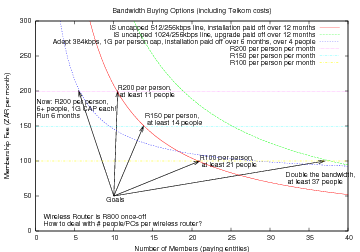
\includegraphics[width=0.8\textwidth]{images/bandwidth-colour.png}
%%%\caption{Planning community bandwidth sharing costs. 
  %%%Note caption capitalization.}
%%%\label{bandwidth} 
% if you move the label it breaks the reference numbering; 
% always have it *after* the caption.
%%%\end{figure}

%%%Remember how to include code with {\tt verbatim} 
%%%and to fix the tabs in {\sf python} in a verbatim environment? 
%%%It may be best to have an `include' command for code, 
%%%not to have to re-edit it all the time.
%%%\verbatimtabinput{code/mycode.py}


